Las arquitecturas o marcos de trabajo que soporten consciencia contextual buscan cumplir ciertos requerimientos por ejemplo abstraer la informaci\'on contextual, ser distribuido e independientes de la aplicaci\'on que las use  \cite{dey1999architecture}, para cubrir estas necesidades se necesita que el marco de trabajo sea accesible por el groupware desde cualquier ubicaci\'on. As\'i la publicaci\'on de servicios web consumibles desde el sistema colaborativo se vuelve una soluci\'ona este problema, con esto se cubre la distribuci\'on de la arquitectura, adem\'as con estos servicios aumenta la compatibilidad con otro tipo de plataformas al enviar sus mensajes serializados o envueltos en una solicitud, haciendo posible la recepci\'on de informaci\'on contextual, compuesta de el estado actual de los elementos de la aplicaci\'on, y la emisi\'on de los resultados hacia el groupware. Con la informaci\'on recibida se mantiene un registro de la actividad del groupware que puede ser \'util para an\'alisis futuros como miner\'ia de datos o reconocimiento de patrones.

Se busca que la arquitectura sea independiente del escenario o dominio de una aplicaci\'on en particular. Por ello, la definici\'on del modelo se divide en dos partes, al igual que \cite{bohu2013} este modelo es presentado con un modelo conceptual y un modelo de dominio de aplicaci\'on; el modelo conceptual est\'a compuesto por entidades que describen una actividad colaborativa mediante relaciones de elementos tales como \textit{actores}, \textit{objetos}, \textit{tareas}, \textit{categor\'ias}, \textit{roles}, \textit{comunidades} y \textit{objetivos}. A partir de este modelo, se pueden identificar elementos con los que se elaborar\'a e instanciar\'a el modelo de dominio de aplicaci\'on, es en esta instanciaci\'on donde se guardar\'an los datos del groupware.

Los datos recibidos deben de ser gestionados en bases de datos y procesados por un motor de razonamiento explicado m\'as adelante, el cu\'al tiene que recibir informaci\'on contextual y tiene que dar como resultado informaci\'on para el usuario o un comando de ejecuci\'on para el groupware. Una vez que se obtienen los resultados se distribuyen a los diferentes dispositivos cliente. Para esto se debe de considerar que al ser las actividades colaborativas los usuarios pueden compartir el contexto en algunas ocasiones, de lo que se desprende la necesidad de agregar la informaci\'on contextual de usuarios que compartan ciertos atributos establecidos para una situaci\'on en particular, es decir, mezclar la informaci\'on de tales usuarios para un manejo de la informaci\'on m\'as eficiente.

\section{Modelo Conceptual}

El presente trabajo hace uso de un modelo conceptual para la representaci\'on de actividades colaborativas dentro de los sistemas groupware, basado un modelo propuesto anteriormente \cite{montane2013context}.  Entre los interactivos se encuentran \textit{actores}, que son los usuarios del sistema, los \textit{objetos} son aquellas entidades que asisten en la realizaci\'on una \textit{tarea} o que son producto de ellas, las \textit{categor\'ias} clasifican a los actores, objetos y tareas, por \'ultimo est\'an los roles, que definen el papel que juega un actor en la actividad y por consecuente sus responsabilidades, los roles pueden ser del objeto o del actor, estos son asignados a una tarea para establecer el rol que va a tener el actor u objeto involucrado en la misma. Los datos cohesivos son de naturaleza abstracta, ya que no se les puede percibir de una forma tangible, entre ellos se encuentran las \textit{equipos} que son asociaciones de actores que colaboran durante una \textit{actividad}, estas actividades representan una unidad de trabajo colaborativo con \textit{metas} que son ideales, en ocasiones inconmensurables, a los que los grupos de trabajo aspiran, por ejemplo ser los mejores realizando una actividad en particular, o ser un equipo de trabajo eficiente, para alcanzar estas \textit{metas} se fijan \textit{objetivos}, que al contrario de las metas, definen medidas que se tienen que satisfacer para decir que estos objetivos han sido cumplidos. En la Figura \ref{cmp:mmc} se observa un modelo conceptual en el que se pueden ver los elementos antes descritos, se refleja la pertenencia de actores a comunidades, comunidades a actividades, las metas que son parte de las actividades y a su vez, los objetivos pertenecientes a cada una de las metas establecidas, y las tareas a realizar para cumplir dichos objetivos; para las tareas y los objetivos se toman en cuenta algunas propiedades \'utiles en el c\'alculo de presencia social como son la asignaci\'on directa a alg\'un actor; la afectaci\'on	de el cumplimiento de la tarea o el objetivo para los usuarios; el resultado generado, es decir a qu\'e magnitud result\'o negativo o positivo; y la efectividad en el caso de las tareas en las que es necesario saber si se llev\'o a cabo correctamente\cite{addCiteHere}.

\begin{figure}[h!]
  \centering
    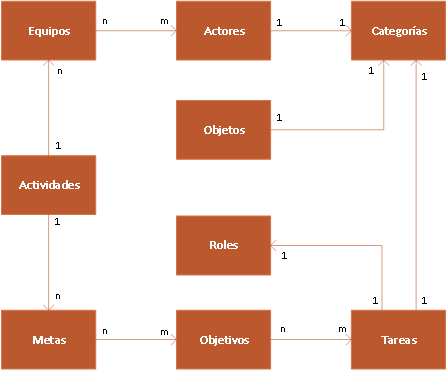
\includegraphics[scale=0.7]{images/MERMetamodel}
  \caption{Modelo Conceptual \cite{montane2013context}}
  \label{cmp:mmc}
\end{figure}


Con este modelo se puede describir el dominio de aplicaciones groupware definiendo cada uno de estos elementos a partir de interacciones, para hacer esto es necesario analizar el groupware y listar los elementos identificados as\'i como sus atributos, estos se 
dar\'an de alta mediante una plataforma web para la definici\'on de dominio que instanciar\'a los datos a un modelo que representar\'a al sistema colaborativo y almacenar\'a las variables contextuales que este transmita a la arquitectura. Cabe mencionar que en este modelo conceptual los elementos cuentan con 3 atributos principales, un identificador del objeto, un nombre descriptivo, y una lista de atributos almacenados en formato JSON, lo que vuelve flexible la forma de registrar y dise\~nar casos de estudio.

\section{Arquitectura}

Para esta arquitectura se tom\'o como modelo base el propuesto por \cite{montane2013context}, la propuesta mostrada en la Figura \ref{ARCH:propuesta}, cuenta con tres capas: recuperaci\'on de datos, gesti\'on de datos, y uso de contexto. Actualmente, en la arquitectura en la que se basa esta propuesta, se ha desarrollado ya la capa de recuperaci\'on de datos y la de gesti\'on, la actual propuesta se concentra principalmente en la tercera capa, la de uso de contexto, teniendo como objetivo implementar un mecanismo de inferencia habilitado para trabajar con el modelo contextual explicado en la secci\'on anterior. Para la primera capa se hace uso de servicios web encargados de recibir la informaci\'on de parte del groupware que despu\'es pasar\'ia a la fase de gesti\'on para ser almacenada; en la segunda capa adem\'as del gestor de datos y las bases de datos est\'a la plataforma web para la especificaci\'on de elementos de dominio y guiones de comportamiento. En la tercera capa se encuentran un motor de inferencia contextual y un in\'erprete de reglas de interacci\'on y servicios que regresan los resultados del motor cuando es necesario.

\newpage

\begin{figure}[h!]
\centering
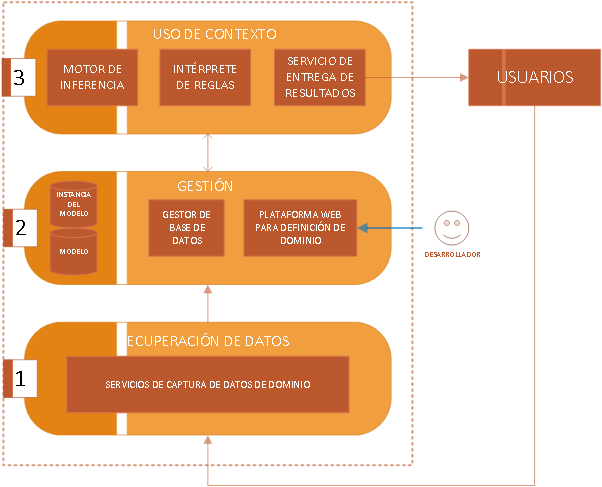
\includegraphics[scale=0.70]{images/arquitecturav2}
\caption{Dise\~o conceptual de la arquitectura}
\label{ARCH:propuesta}
\end{figure}

\begin{enumerate}


\item \textbf{Recuperac\'on de datos}. Se captura informaci\'on contextual enviada por el groupware por medio de servicios web publicados para la comunicaci\'on entre la arquitectura y el sistema, estos servicios son generados a partir del modelo especificado en la plataforma web de la segunda capa, as\'i mismo se encuentra un servicio que captura las ejecuciones de tareas durante una actividad en el groupware, los datos son enviados en un formato espec\'ifico para que capas superiores puedan procesarla.

\item \textbf{Gesti\'on}. Aunque es trivial en este caso, es necesario tener m\'etodos de actualizaci\'on y recuperai\'on de datos contextuales de las bases de datos, adem\'as a este nivel est\'a definido el modelo conceptual y la plataforma web mostrada en la Figura \ref{arch:wplatform}.

\newpage
\begin{figure}[h!]
\centering
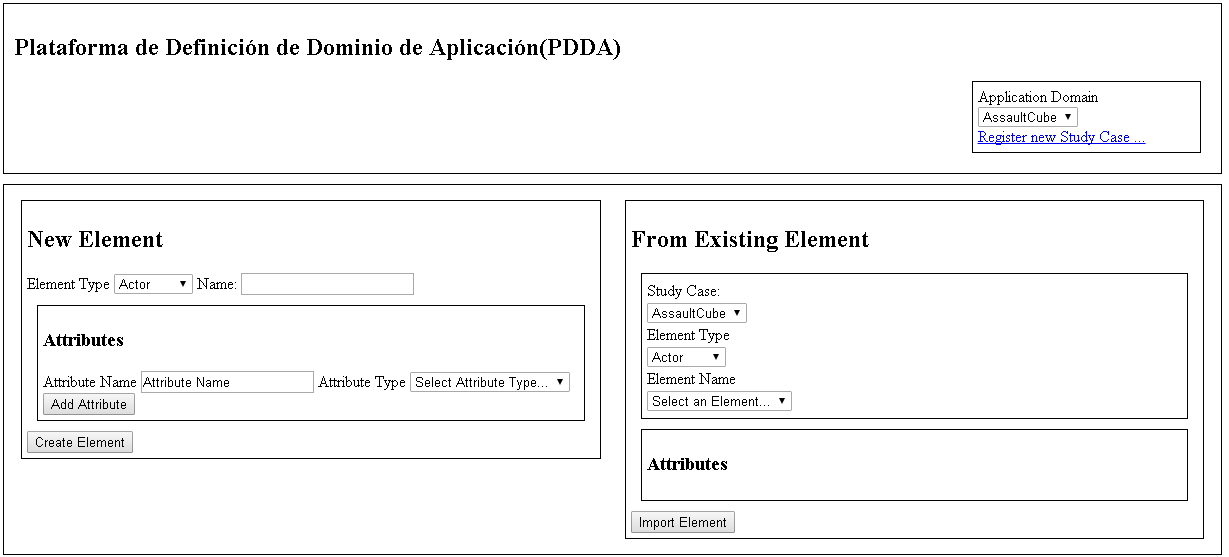
\includegraphics[scale=0.50]{images/attDef}
\caption{Plataforma web de Definici\'on de Dominio de Aplicaci\'on}
\label{arch:wplatform}
\end{figure}

En esta platafaorma se encuentran formularios en los que se define cada elemento con un nombre y con una lista de atributos, de esta forma se define el modelo de dominio de la aplicaci\'on, detallando los datos de cada elemento del dominio, despu\'es, en la misma plataforma web, se definen el conjunto de reglas para adaptar el groupware a la actividad de los usuarios, estas reglas ser\'an explicadas m\'as adelante. Con la definici\'on del modelo de dominio se dan de alta los servicios mencionados en el punto anterior. Este proceso de definici\'on de modelo de dominio se describe en la Figura \ref{arch:domdef}

\begin{figure}[h!]
\centering
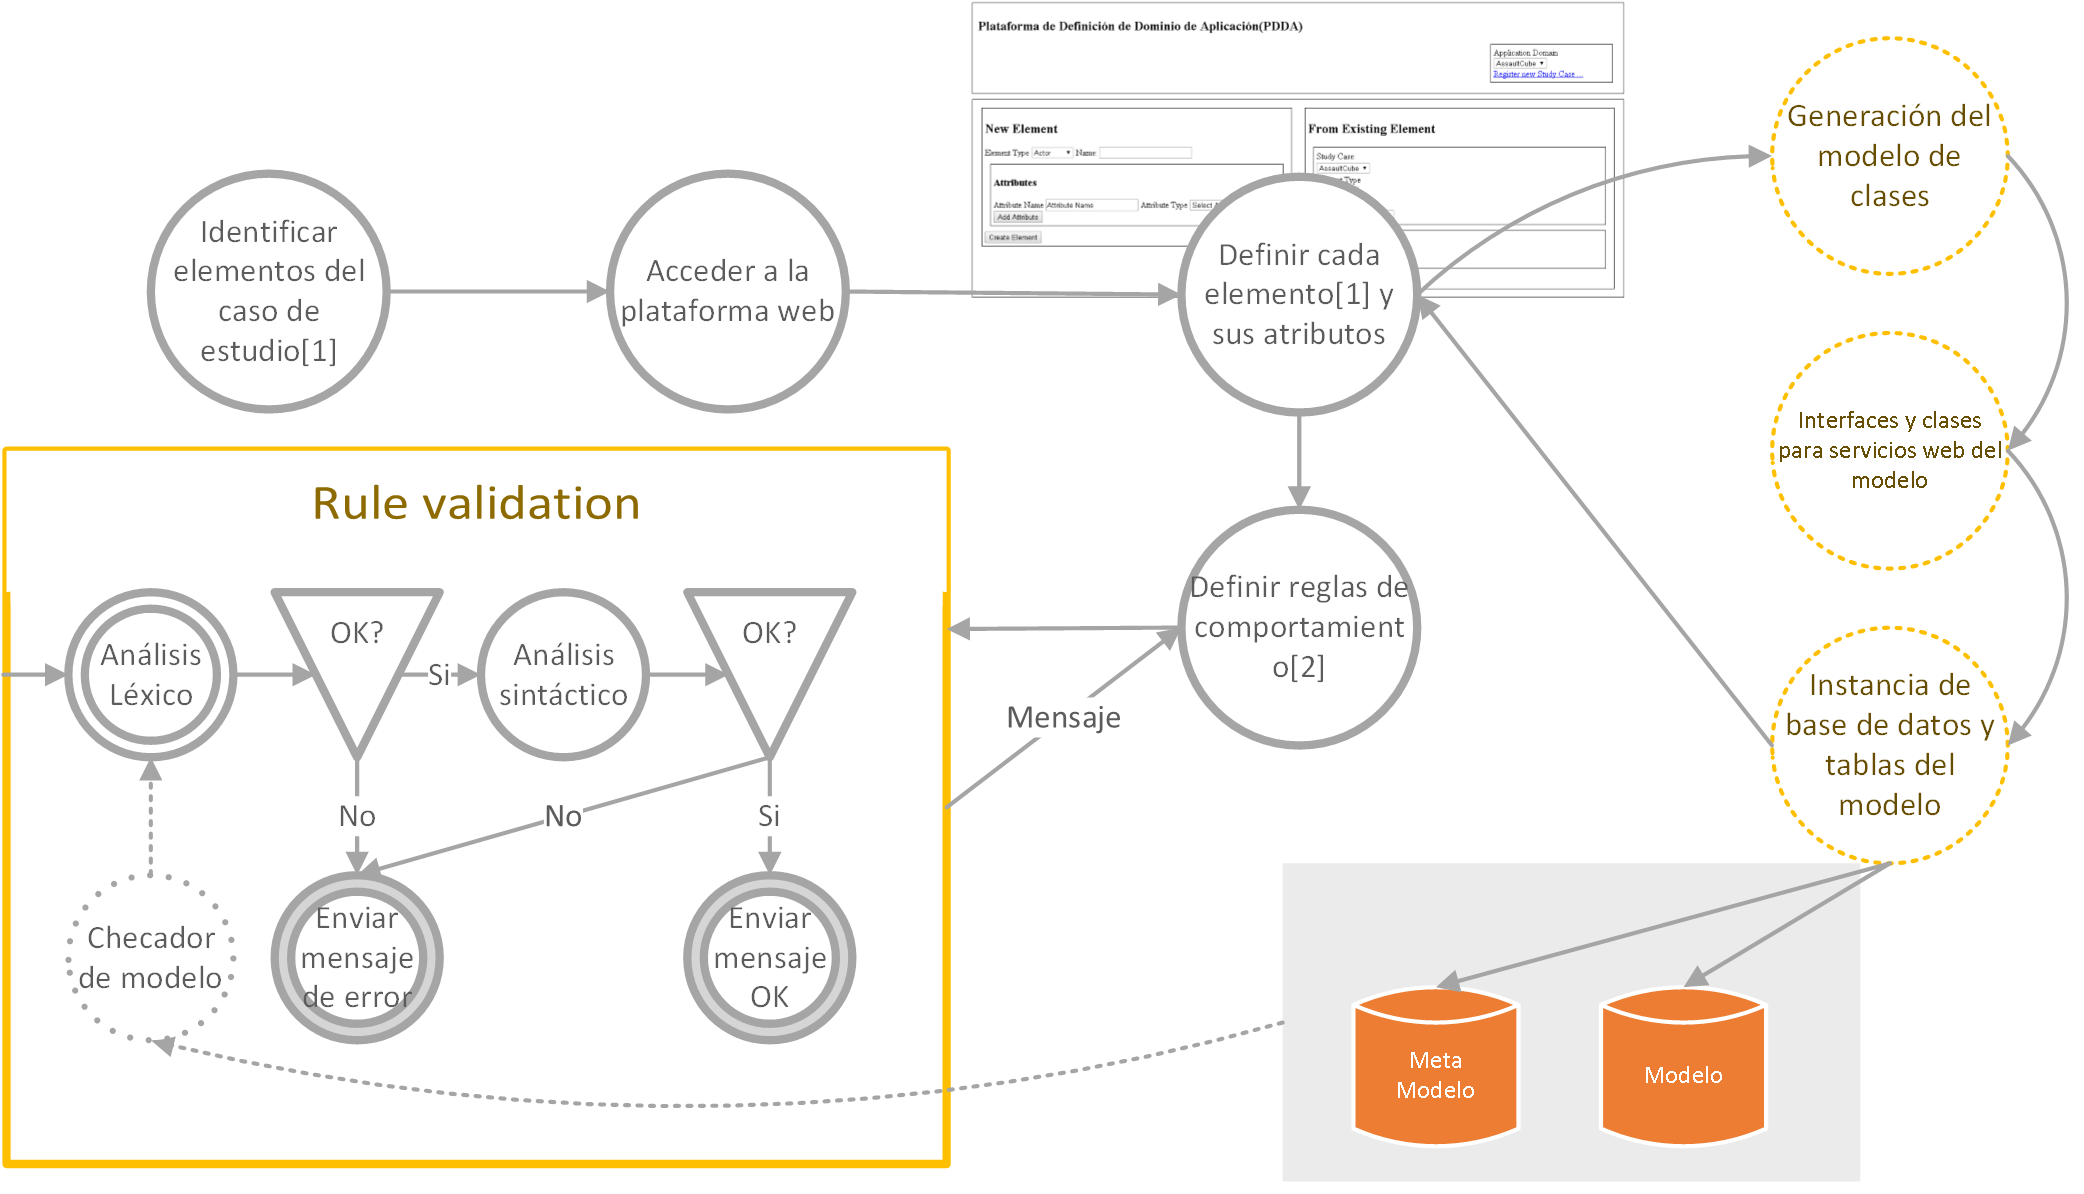
\includegraphics[scale=0.7]{images/ModelDefinitionByWebPlatformProcess_ESP}
\caption{Proceso para definir modelo de dominio y reglas de comportamiento.}
\label{arch:domdef}
\end{figure}

\item \textbf{Uso de contexto}. En esta \'ultima capa se encuentra un int\'erprete de reglas y un motor de inferencia, el int\'erprete se encarga de verificar la sintaxis, realizar un an\'alisis sem\'antico e identificar los elementos de cada regla, y verificar que estos elementos existan en el modelo de dominio, todo esto con ayuda de m\'etodos de an\'alisis como un aut\'omata y expresiones regulares. El int\'erprete es usado por la plataforma web para validar las reglas que escriba el desarrollador en los guiones, una vez verificadas, se guardan junto con los guiones para que pueda usarlos el motor de inferencia. El motor de inferencia tambi\'en hace uso de el int\'erprete para validar estructuras similares a las reglas, estas son las ejecuciones de las tareas que se llevan a cabo durante una actividad. El motor llevar\'a la cuenta de las frecuencias de estas ejecuciones y las comparar\'a con las establecidas en los guiones, una ves que un gui\'on se cumple, se recuperan los resultados y se reenv\'ian a trav\'es de servicios de distribuci\'on de informaci\'on.

\end{enumerate}


Despu\'es de definir el modelo en la plataforma, se especif\'ican los guiones, los cuales son un conjunto de reglas que describen las interacciones que se llevan a cabo dentro de el groupware y las caracter\'isticas de un actor de a cuerdo a patrones de comportamiento particulares, con estos guiones se vigila la actividad de los usuarios y dependiendo de las tareas y el estado de los usuarios se tomar\'an medidas, tambi\'en incluidas en las reglas, para hacer que el groupware responda a ese comportamiento, un ejemplo ser\'ia un guion para un sistema gu\'ia de turistas en el que se podr\'ia definir el comportamiento para una persona extraviada por la falta de conocimiento del lugar, definiendo reglas que verifiquen el n\'umero de consultas sobre ubicaci\'ones de lugares de inter\'es, la ubicaci\'on actual del turista en relaci\'on con estos lugares, la frecuencia con la que el turista llega con retardo a los eventos, etc. 

\section{Motor de inferencia contextual}

Este trabajo en particular se centra en el dise\~o e implementaci\'on de la capa de uso de contexto mencionada en la secci\'on anterior, para eso se proponen tres m\'odulos principales: un int\'erprete para el lenguaje de reglas que se propone para describir el contexto de los usuarios durante una actividad colaborativa, un motor de reglas que apoy\'andose de las reglas definidas infiere las medidas a tomar para las situaciones descritas por las reglas y un servicio de entrega de resultados que se dispara cuando el motor de inferencia obtiene alg\'un resultado.

El int\'erprete valida la definici\'on de las reglas con un lenguaje que implementa un aut\'omata de estado finito y expresiones regulares creadas para este prop\'osito, con ellas se describe la pertenencia o relaci\'on de alguno de los elementos o instancias al otro en el modelo, comparan valores con los de los atributos de los elementos para condicionar su estado actual, o permiten representar la ejecuci\'on de tareas realizadas por actores en las que se puede incluir un elemento de asistencia, adem\'as se puede revisar el estado de estas ejecuciones comparando alg\'un atributo de la tarea con un valor dado, por ejemplo el saber si una tarea fue exitosa o fallida. Estos tres tipos de reglas se definen como sigue.

\begin{itemize}
\item Pertenencia(P): $Elemento \rightarrow Elemento$ para validar que un elemento pertenezca a otro, o $Elemento \rightsquigarrow Elemento$ para validar que no pertenezca.

\item Comparaci\'on(C): $ Elemento.Atributo[<=>¬]Valor $ para validar que el atributo de un elemento cumpla con la condici\'on impuesta.

\item Ejecuci\'on(X): indica que una tarea ha sido llevada a cabo, y si es el caso, con qu\'e objeto se realiz\'o, adem\'as se puede puntualizar otras caracter\'isticas de la tarea como efectividad, o la afectaci\'on que tuvo, y si es necesario se puede a\~nadir una regla de pertenencia en la misma declaraci\'on del elemento.  $ [Elemento | P] - Tarea(nombre, Elemento).nombreAtributo [ = | \neg | < | > ] valor $; un ejemplo pr\'actico de esta regla puede ser la ejecuci\'on de un disparo efectivo por parte de un jugador perteneciente al equipo rojo con un francotirador.
\end{itemize}

En donde $Elemento$ es un elemento del modelo descrito por un elemento conceptual, un elemento del dominio, y la instancia o instancias quedando la sintaxis de la siguiente forma: $Concepto(Dominio{ListaDeInstancias})$, evidentemente los elementos y las instancias tienen que formar parte del modelo.

Para escribir un gui\'on se usan varias reglas concatenadas que sirvan para describir el comportamiento de un usuario y una consecuencia que ser\'a el resultado que contiene ejecuciones de tareas que el groupware recibir\'a, interpretar\'a y adaptar\'a. Un gui\'on tiene la siguiente forma.


\begin{table}
\fontsize{9}{6}
\label{guion:structure}
\centering
\begin{tabular}{|p{8cm}|l|l|}
\hline \textbf{Regla} & \textbf{Tipo} & \textbf{Frecuencia} \\ 
\hline $Elem_1(DomEl_a\{*\})\rightarrow Elem_2(DomEl_b)$ & pertenencia & no aplica \\ 
\hline \& 
$Elem_1(DomEl_a\{instancia_1\}).Nombre=Ana$ & comparaci\'on & no aplica \\ 
\hline \& $Elem_1(DomElem_a\{instancia_1\})-Task(escribir, Objetos(lapiz)).tiempo=2segundos$ & ejecuci\'on & 5 \\ 
\hline \multicolumn{3}{|c|}{$:=$} \\  
\hline $ME(DE\{i_1,i_2,i_3,...,i_n\})-Task(mostrarMensaje)$ & tarea resultante & no aplica \\ 
\hline 
\end{tabular} 

\end{table}

En este gui\'on(Figura \ref{guion:structure}) se muestra un ejemplo de cada uno de los tipos de reglas descritos antes, cabe mencionar que el \'unico tipo de regla en el que se especifica una frecuencia es en la ejecuci\'on de tareas, ya que no tiene sentido hacerlo para las otras dos porque son comparaciones de estados de o propiedades de elementos.

El motor de inferencia recupera los guiones y los usa como una lsta de verificaci\'on para proporcionar informaci\'on de inter\'es para los usuarios o comandos de ejecuci\'on para la adaptaci\'on del sistema a la situaci\'on actual. Dentro del motor se har\'a una instancia de los guiones recuperados del modelo de dominio, la arquitectura estar\'a recibiendo ejecuciones de tareas durante la actividad del groupware de manera constante cada cierto tiempo, estas tareas ser\'an comparadas con cada uno de los guiones y se llevar\'a un conteo de la frecuencia de cada una de ellas, cuando las ejecuciones lleguen al n\'umero indicado, el guion se cumple y se manda otra tarea, tambi\'en incluida en el gui\'on, como resultado para que ser\'a interpretada y ejecutada en el groupware. Una vez que se cumple un guion, este se reinicia para continuar recibiendo las tareas desde el sistema. Con esto se pueden ofrecer resultados coherentes al tiempo en el que el sistema se ejecuta. Los resultados obtenidos son gestionados por un administrador de resultados que almacena los datos en una base de datos para mantener registro hist\'orico del comportamiento del groupware. Una vez obtenidos y almacenados los resultados un servicio de distribuci\'on de datos se encarga de enviar la informaci\'on al groupware con los resultados. Este proceso es iterativo, ya que vive por el tiempo en el que el groupware opera.  El proceso del motor se puede ver reflejado en la Figura \ref{arch:useofcontext}

\begin{figure}[h!]
\centering
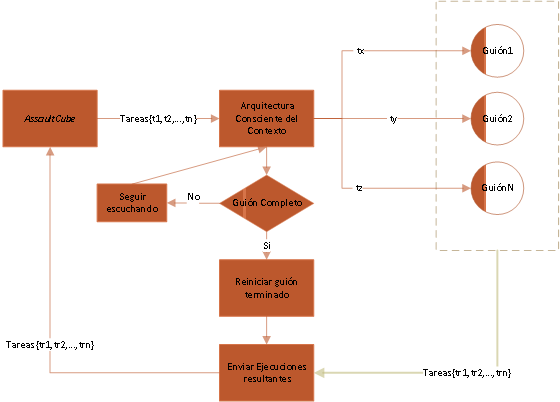
\includegraphics[scale=0.80]{images/RunningProcess_ESP}
\caption{Proceso de inferencia}
\label{arch:useofcontext}
\end{figure}